\documentclass{standalone}
\usepackage{tikz}
\usetikzlibrary{patterns, positioning}


\begin{document}
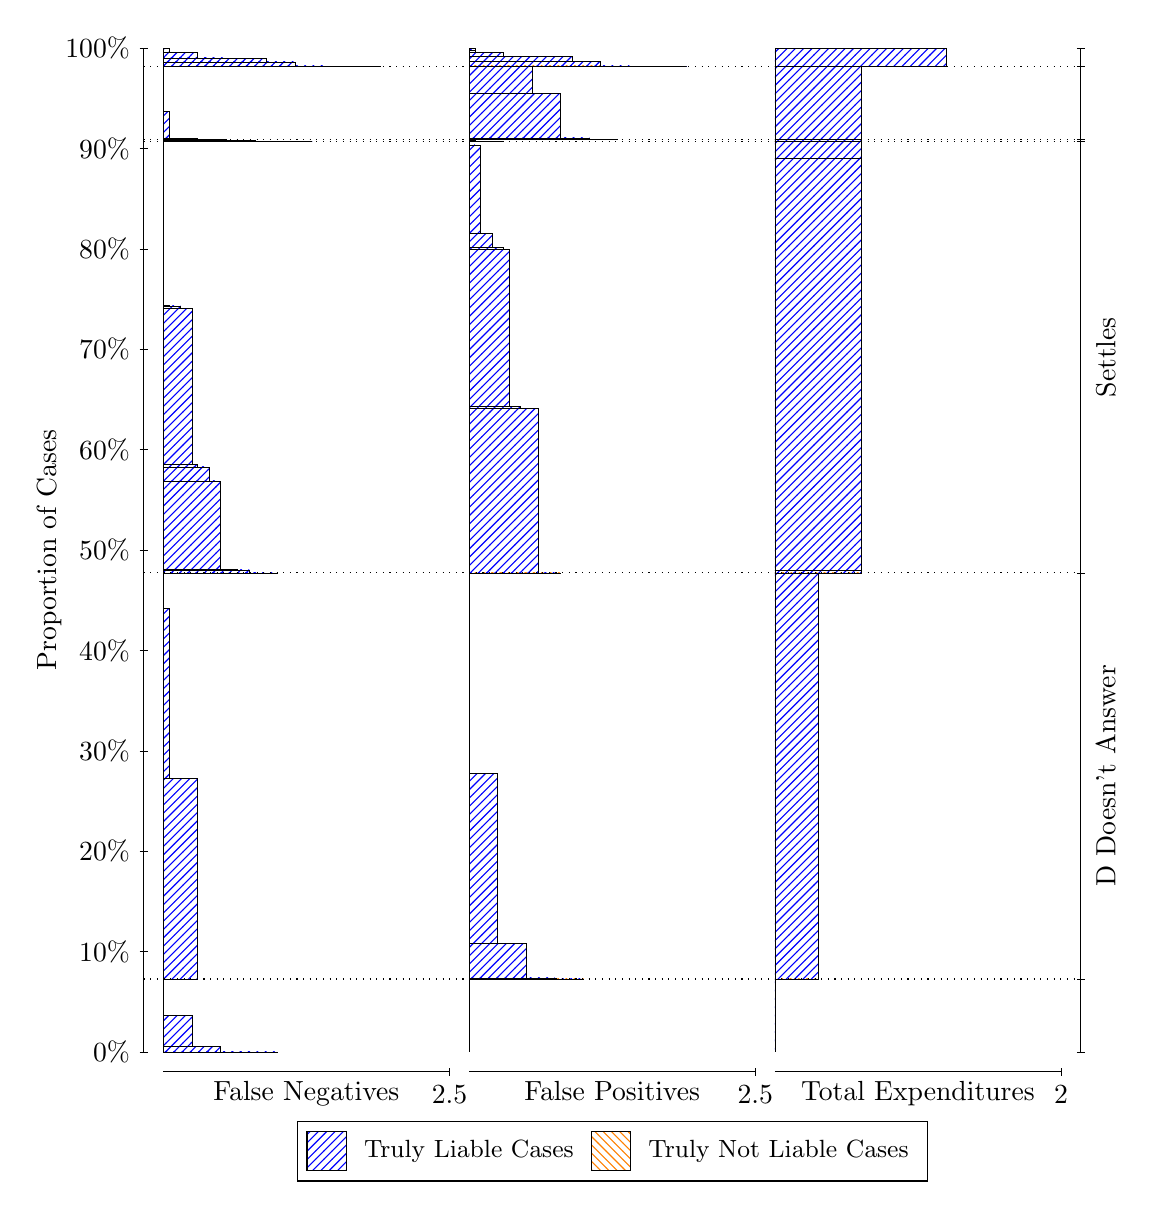
\begin{tikzpicture}
\draw[black, very thin] (1.5,1.75) -- (1.5,14.5);
\node[rotate=90, text=black, anchor=center] at (0.3, 8.125) {Proportion of Cases};
\draw[black, very thin] (1.45,1.75) -- (1.55,1.75);
\node[text=black, anchor=east] at (1.45, 1.75) {0\%};
\draw[black, very thin] (1.45,3.025) -- (1.55,3.025);
\node[text=black, anchor=east] at (1.45, 3.025) {10\%};
\draw[black, very thin] (1.45,4.3) -- (1.55,4.3);
\node[text=black, anchor=east] at (1.45, 4.3) {20\%};
\draw[black, very thin] (1.45,5.575) -- (1.55,5.575);
\node[text=black, anchor=east] at (1.45, 5.575) {30\%};
\draw[black, very thin] (1.45,6.85) -- (1.55,6.85);
\node[text=black, anchor=east] at (1.45, 6.85) {40\%};
\draw[black, very thin] (1.45,8.125) -- (1.55,8.125);
\node[text=black, anchor=east] at (1.45, 8.125) {50\%};
\draw[black, very thin] (1.45,9.4) -- (1.55,9.4);
\node[text=black, anchor=east] at (1.45, 9.4) {60\%};
\draw[black, very thin] (1.45,10.675) -- (1.55,10.675);
\node[text=black, anchor=east] at (1.45, 10.675) {70\%};
\draw[black, very thin] (1.45,11.95) -- (1.55,11.95);
\node[text=black, anchor=east] at (1.45, 11.95) {80\%};
\draw[black, very thin] (1.45,13.225) -- (1.55,13.225);
\node[text=black, anchor=east] at (1.45, 13.225) {90\%};
\draw[black, very thin] (1.45,14.5) -- (1.55,14.5);
\node[text=black, anchor=east] at (1.45, 14.5) {100\%};

\draw[black, very thin] (13.4,1.75) -- (13.4,14.5);
\draw[black, very thin] (13.35,1.75) -- (13.45,1.75);
\node[anchor=west] at (13.35, 1.75) {};
\draw[black, very thin] (13.35,2.6771) -- (13.45,2.6771);
\node[anchor=west] at (13.35, 2.6771) {};
\draw[black, very thin] (13.35,7.8343) -- (13.45,7.8343);
\node[anchor=west] at (13.35, 7.8343) {};
\draw[black, very thin] (13.35,13.314) -- (13.45,13.314);
\node[anchor=west] at (13.35, 13.314) {};
\draw[black, very thin] (13.35,13.344) -- (13.45,13.344);
\node[anchor=west] at (13.35, 13.344) {};
\draw[black, very thin] (13.35,14.269) -- (13.45,14.269);
\node[anchor=west] at (13.35, 14.269) {};
\draw[black, very thin] (13.35,14.5) -- (13.45,14.5);
\node[anchor=west] at (13.35, 14.5) {};

\draw[black, very thin, pattern color=blue, pattern=north east lines] (1.75,1.75) rectangle (3.2033,1.75);
\draw[black, very thin, pattern color=blue, pattern=north east lines] (1.75,1.75) rectangle (2.84,1.7506);
\draw[black, very thin, pattern color=blue, pattern=north east lines] (1.75,1.7506) rectangle (2.4767,1.8242);
\draw[black, very thin, pattern color=blue, pattern=north east lines] (1.75,1.8242) rectangle (2.1133,2.2142);
\draw[black, very thin, pattern color=orange, pattern=north west lines] (1.75,2.2142) rectangle (1.75,2.2142);
\draw[black, very thin, pattern color=blue, pattern=north east lines] (1.75,2.2142) rectangle (1.75,2.6771);
\draw[black, very thin, pattern color=blue, pattern=north east lines] (1.75,2.6771) rectangle (2.186,5.223);
\draw[black, very thin, pattern color=blue, pattern=north east lines] (1.75,5.223) rectangle (1.8227,7.3786);
\draw[black, very thin, pattern color=orange, pattern=north west lines] (1.75,7.3786) rectangle (1.75,7.3786);
\draw[black, very thin, pattern color=blue, pattern=north east lines] (1.75,7.3786) rectangle (1.75,7.8343);
\draw[black, very thin, pattern color=blue, pattern=north east lines] (1.75,7.8343) rectangle (3.2033,7.8343);
\draw[black, very thin, pattern color=blue, pattern=north east lines] (1.75,7.8343) rectangle (3.058,7.8344);
\draw[black, very thin, pattern color=blue, pattern=north east lines] (1.75,7.8344) rectangle (2.9127,7.8344);
\draw[black, very thin, pattern color=blue, pattern=north east lines] (1.75,7.8344) rectangle (2.84,7.8711);
\draw[black, very thin, pattern color=blue, pattern=north east lines] (1.75,7.8711) rectangle (2.6947,7.8796);
\draw[black, very thin, pattern color=blue, pattern=north east lines] (1.75,7.8796) rectangle (2.5493,7.881);
\draw[black, very thin, pattern color=blue, pattern=north east lines] (1.75,7.881) rectangle (2.4767,9.0025);
\draw[black, very thin, pattern color=blue, pattern=north east lines] (1.75,9.0025) rectangle (2.3313,9.1795);
\draw[black, very thin, pattern color=blue, pattern=north east lines] (1.75,9.1795) rectangle (2.186,9.2092);
\draw[black, very thin, pattern color=blue, pattern=north east lines] (1.75,9.2092) rectangle (2.1133,11.198);
\draw[black, very thin, pattern color=blue, pattern=north east lines] (1.75,11.198) rectangle (1.968,11.225);
\draw[black, very thin, pattern color=blue, pattern=north east lines] (1.75,11.225) rectangle (1.8227,11.229);
\draw[black, very thin, pattern color=orange, pattern=north west lines] (1.75,11.229) rectangle (1.75,11.229);
\draw[black, very thin, pattern color=blue, pattern=north east lines] (1.75,11.229) rectangle (1.75,13.314);
\draw[black, very thin, pattern color=blue, pattern=north east lines] (1.75,13.314) rectangle (3.6393,13.314);
\draw[black, very thin, pattern color=blue, pattern=north east lines] (1.75,13.314) rectangle (3.276,13.314);
\draw[black, very thin, pattern color=blue, pattern=north east lines] (1.75,13.314) rectangle (2.9127,13.325);
\draw[black, very thin, pattern color=blue, pattern=north east lines] (1.75,13.325) rectangle (2.5493,13.344);
\draw[black, very thin, pattern color=blue, pattern=north east lines] (1.75,13.344) rectangle (2.186,13.344);
\draw[black, very thin, pattern color=orange, pattern=north west lines] (1.75,13.344) rectangle (1.75,13.344);
\draw[black, very thin, pattern color=blue, pattern=north east lines] (1.75,13.344) rectangle (2.186,13.348);
\draw[black, very thin, pattern color=blue, pattern=north east lines] (1.75,13.348) rectangle (1.8227,13.692);
\draw[black, very thin, pattern color=orange, pattern=north west lines] (1.75,13.692) rectangle (1.75,13.692);
\draw[black, very thin, pattern color=blue, pattern=north east lines] (1.75,13.692) rectangle (1.75,14.269);
\draw[black, very thin, pattern color=blue, pattern=north east lines] (1.75,14.269) rectangle (4.5113,14.269);
\draw[black, very thin, pattern color=blue, pattern=north east lines] (1.75,14.269) rectangle (4.148,14.269);
\draw[black, very thin, pattern color=blue, pattern=north east lines] (1.75,14.269) rectangle (3.7847,14.272);
\draw[black, very thin, pattern color=blue, pattern=north east lines] (1.75,14.272) rectangle (3.4213,14.324);
\draw[black, very thin, pattern color=blue, pattern=north east lines] (1.75,14.324) rectangle (3.276,14.324);
\draw[black, very thin, pattern color=blue, pattern=north east lines] (1.75,14.324) rectangle (3.058,14.372);
\draw[black, very thin, pattern color=blue, pattern=north east lines] (1.75,14.372) rectangle (2.9127,14.372);
\draw[black, very thin, pattern color=blue, pattern=north east lines] (1.75,14.372) rectangle (2.6947,14.373);
\draw[black, very thin, pattern color=blue, pattern=north east lines] (1.75,14.373) rectangle (2.5493,14.374);
\draw[black, very thin, pattern color=blue, pattern=north east lines] (1.75,14.374) rectangle (2.3313,14.374);
\draw[black, very thin, pattern color=blue, pattern=north east lines] (1.75,14.374) rectangle (2.186,14.374);
\draw[black, very thin, pattern color=blue, pattern=north east lines] (1.75,14.374) rectangle (2.186,14.441);
\draw[black, very thin, pattern color=blue, pattern=north east lines] (1.75,14.441) rectangle (1.8227,14.442);
\draw[black, very thin, pattern color=blue, pattern=north east lines] (1.75,14.442) rectangle (1.8227,14.495);
\draw[black, very thin, pattern color=orange, pattern=north west lines] (1.75,14.495) rectangle (1.75,14.495);
\draw[black, very thin, pattern color=blue, pattern=north east lines] (1.75,14.495) rectangle (1.75,14.5);
\draw[black, very thin, pattern color=orange, pattern=north west lines] (5.6333,1.75) rectangle (5.6333,1.75);
\draw[black, very thin, pattern color=blue, pattern=north east lines] (5.6333,1.75) rectangle (5.6333,2.6771);
\draw[black, very thin, pattern color=orange, pattern=north west lines] (5.6333,2.6771) rectangle (7.0867,2.6771);
\draw[black, very thin, pattern color=blue, pattern=north east lines] (5.6333,2.6771) rectangle (7.0867,2.6772);
\draw[black, very thin, pattern color=blue, pattern=north east lines] (5.6333,2.6772) rectangle (6.7233,2.6913);
\draw[black, very thin, pattern color=blue, pattern=north east lines] (5.6333,2.6913) rectangle (6.36,3.1328);
\draw[black, very thin, pattern color=blue, pattern=north east lines] (5.6333,3.1328) rectangle (5.9967,5.2884);
\draw[black, very thin, pattern color=blue, pattern=north east lines] (5.6333,5.2884) rectangle (5.6333,7.8343);
\draw[black, very thin, pattern color=orange, pattern=north west lines] (5.6333,7.8343) rectangle (6.796,7.8343);
\draw[black, very thin, pattern color=blue, pattern=north east lines] (5.6333,7.8343) rectangle (6.796,7.8344);
\draw[black, very thin, pattern color=orange, pattern=north west lines] (5.6333,7.8344) rectangle (6.6507,7.8344);
\draw[black, very thin, pattern color=blue, pattern=north east lines] (5.6333,7.8344) rectangle (6.6507,7.8344);
\draw[black, very thin, pattern color=orange, pattern=north west lines] (5.6333,7.8344) rectangle (6.5053,7.8344);
\draw[black, very thin, pattern color=blue, pattern=north east lines] (5.6333,7.8344) rectangle (6.5053,9.9197);
\draw[black, very thin, pattern color=blue, pattern=north east lines] (5.6333,9.9197) rectangle (6.4327,9.9241);
\draw[black, very thin, pattern color=blue, pattern=north east lines] (5.6333,9.9241) rectangle (6.2873,9.9506);
\draw[black, very thin, pattern color=blue, pattern=north east lines] (5.6333,9.9506) rectangle (6.142,11.939);
\draw[black, very thin, pattern color=blue, pattern=north east lines] (5.6333,11.939) rectangle (6.0693,11.969);
\draw[black, very thin, pattern color=blue, pattern=north east lines] (5.6333,11.969) rectangle (5.924,12.146);
\draw[black, very thin, pattern color=blue, pattern=north east lines] (5.6333,12.146) rectangle (5.7787,13.268);
\draw[black, very thin, pattern color=blue, pattern=north east lines] (5.6333,13.268) rectangle (5.706,13.269);
\draw[black, very thin, pattern color=blue, pattern=north east lines] (5.6333,13.269) rectangle (5.6333,13.314);
\draw[black, very thin, pattern color=orange, pattern=north west lines] (5.6333,13.314) rectangle (6.0693,13.314);
\draw[black, very thin, pattern color=blue, pattern=north east lines] (5.6333,13.314) rectangle (6.0693,13.315);
\draw[black, very thin, pattern color=blue, pattern=north east lines] (5.6333,13.315) rectangle (5.706,13.334);
\draw[black, very thin, pattern color=blue, pattern=north east lines] (5.6333,13.334) rectangle (5.6333,13.344);
\draw[black, very thin, pattern color=orange, pattern=north west lines] (5.6333,13.344) rectangle (7.5227,13.344);
\draw[black, very thin, pattern color=blue, pattern=north east lines] (5.6333,13.344) rectangle (7.5227,13.344);
\draw[black, very thin, pattern color=blue, pattern=north east lines] (5.6333,13.344) rectangle (7.1593,13.36);
\draw[black, very thin, pattern color=blue, pattern=north east lines] (5.6333,13.36) rectangle (6.796,13.921);
\draw[black, very thin, pattern color=blue, pattern=north east lines] (5.6333,13.921) rectangle (6.4327,14.265);
\draw[black, very thin, pattern color=blue, pattern=north east lines] (5.6333,14.265) rectangle (6.0693,14.269);
\draw[black, very thin, pattern color=orange, pattern=north west lines] (5.6333,14.269) rectangle (8.3947,14.269);
\draw[black, very thin, pattern color=blue, pattern=north east lines] (5.6333,14.269) rectangle (8.3947,14.269);
\draw[black, very thin, pattern color=orange, pattern=north west lines] (5.6333,14.269) rectangle (8.0313,14.269);
\draw[black, very thin, pattern color=blue, pattern=north east lines] (5.6333,14.269) rectangle (8.0313,14.269);
\draw[black, very thin, pattern color=orange, pattern=north west lines] (5.6333,14.269) rectangle (7.668,14.269);
\draw[black, very thin, pattern color=blue, pattern=north east lines] (5.6333,14.269) rectangle (7.668,14.274);
\draw[black, very thin, pattern color=orange, pattern=north west lines] (5.6333,14.274) rectangle (7.3047,14.274);
\draw[black, very thin, pattern color=blue, pattern=north east lines] (5.6333,14.274) rectangle (7.3047,14.327);
\draw[black, very thin, pattern color=blue, pattern=north east lines] (5.6333,14.327) rectangle (6.9413,14.395);
\draw[black, very thin, pattern color=orange, pattern=north west lines] (5.6333,14.395) rectangle (6.796,14.395);
\draw[black, very thin, pattern color=blue, pattern=north east lines] (5.6333,14.395) rectangle (6.796,14.395);
\draw[black, very thin, pattern color=blue, pattern=north east lines] (5.6333,14.395) rectangle (6.578,14.396);
\draw[black, very thin, pattern color=orange, pattern=north west lines] (5.6333,14.396) rectangle (6.4327,14.396);
\draw[black, very thin, pattern color=blue, pattern=north east lines] (5.6333,14.396) rectangle (6.4327,14.397);
\draw[black, very thin, pattern color=blue, pattern=north east lines] (5.6333,14.397) rectangle (6.2147,14.397);
\draw[black, very thin, pattern color=blue, pattern=north east lines] (5.6333,14.397) rectangle (6.0693,14.444);
\draw[black, very thin, pattern color=orange, pattern=north west lines] (5.6333,14.444) rectangle (6.0693,14.444);
\draw[black, very thin, pattern color=blue, pattern=north east lines] (5.6333,14.444) rectangle (6.0693,14.445);
\draw[black, very thin, pattern color=blue, pattern=north east lines] (5.6333,14.445) rectangle (5.8513,14.445);
\draw[black, very thin, pattern color=blue, pattern=north east lines] (5.6333,14.445) rectangle (5.706,14.475);
\draw[black, very thin, pattern color=blue, pattern=north east lines] (5.6333,14.475) rectangle (5.706,14.497);
\draw[black, very thin, pattern color=blue, pattern=north east lines] (5.6333,14.497) rectangle (5.6333,14.5);
\draw[black, very thin, pattern color=orange, pattern=north west lines] (9.5167,1.75) rectangle (9.5167,1.75);
\draw[black, very thin, pattern color=blue, pattern=north east lines] (9.5167,1.75) rectangle (9.5167,2.6771);
\draw[black, very thin, pattern color=orange, pattern=north west lines] (9.5167,2.6771) rectangle (10.062,2.6771);
\draw[black, very thin, pattern color=blue, pattern=north east lines] (9.5167,2.6771) rectangle (10.062,7.8343);
\draw[black, very thin, pattern color=orange, pattern=north west lines] (9.5167,7.8343) rectangle (10.607,7.8343);
\draw[black, very thin, pattern color=blue, pattern=north east lines] (9.5167,7.8343) rectangle (10.607,7.8699);
\draw[black, very thin, pattern color=orange, pattern=north west lines] (9.5167,7.8699) rectangle (10.607,7.8699);
\draw[black, very thin, pattern color=blue, pattern=north east lines] (9.5167,7.8699) rectangle (10.607,13.102);
\draw[black, very thin, pattern color=orange, pattern=north west lines] (9.5167,13.102) rectangle (10.607,13.102);
\draw[black, very thin, pattern color=blue, pattern=north east lines] (9.5167,13.102) rectangle (10.607,13.314);
\draw[black, very thin, pattern color=orange, pattern=north west lines] (9.5167,13.314) rectangle (10.607,13.314);
\draw[black, very thin, pattern color=blue, pattern=north east lines] (9.5167,13.314) rectangle (10.607,13.344);
\draw[black, very thin, pattern color=orange, pattern=north west lines] (9.5167,13.344) rectangle (10.607,13.344);
\draw[black, very thin, pattern color=blue, pattern=north east lines] (9.5167,13.344) rectangle (10.607,14.269);
\draw[black, very thin, pattern color=orange, pattern=north west lines] (9.5167,14.269) rectangle (11.697,14.269);
\draw[black, very thin, pattern color=blue, pattern=north east lines] (9.5167,14.269) rectangle (11.697,14.5);
\draw[black, dotted] (1.5,2.6771) -- (13.4,2.6771);
\draw[black, dotted] (1.5,7.8343) -- (13.4,7.8343);
\draw[black, dotted] (1.5,13.314) -- (13.4,13.314);
\draw[black, dotted] (1.5,13.344) -- (13.4,13.344);
\draw[black, dotted] (1.5,14.269) -- (13.4,14.269);
\draw[black, very thin] (1.75,1.5) -- (5.3833,1.5);
\node[text=black, anchor=north] at (3.5667, 1.5) {False Negatives};
\draw[black, very thin] (5.3833,1.45) -- (5.3833,1.55);
\node[text=black, anchor=north] at (5.3833, 1.45) {2.5};

\draw[black, very thin] (5.6333,1.5) -- (9.2667,1.5);
\node[text=black, anchor=north] at (7.45, 1.5) {False Positives};
\draw[black, very thin] (9.2667,1.45) -- (9.2667,1.55);
\node[text=black, anchor=north] at (9.2667, 1.45) {2.5};

\draw[black, very thin] (9.5167,1.5) -- (13.15,1.5);
\node[text=black, anchor=north] at (11.333, 1.5) {Total Expenditures};
\draw[black, very thin] (13.15,1.45) -- (13.15,1.55);
\node[text=black, anchor=north] at (13.15, 1.45) {2};


\node[text=black, centered, rotate=90] at (13.72, 5.2557) {D Doesn't Answer};
\node[text=black, centered, rotate=90] at (13.72, 10.574) {Settles};




\draw (7.449999999999999,1.5) node[draw=none] (baseCoordinate) {};
\begin{scope}[align=center]
        \matrix[scale=0.5, draw=black, below=0.5cm of baseCoordinate, nodes={draw}, column sep=0.1cm]{
            \node[rectangle, draw, minimum width=0.5cm, minimum height=0.5cm, pattern color=blue, pattern=north east lines] {}; &
            \node[draw=none, font=\small, text=black] (B) {Truly Liable Cases}; &
            \node[rectangle, draw, minimum width=0.5cm, minimum height=0.5cm, pattern color=orange, pattern=north west lines] {}; &
            \node[draw=none, font=\small, text=black] (B) {Truly Not Liable Cases}; \\
            };
\end{scope}

\end{tikzpicture}
\end{document}